\documentclass[11pt]{article}
\usepackage[margin=1in]{geometry}
\usepackage{mathpazo}
\usepackage{amsmath,amssymb}
\usepackage{microtype}
\usepackage{booktabs}
\usepackage{graphicx}
\usepackage[dvipsnames]{xcolor}
\usepackage{tikz}
\usetikzlibrary{positioning,arrows.meta,calc,fit,backgrounds}
\usepackage[most]{tcolorbox}
\usepackage{enumitem}
\usepackage{listings}
\usepackage[font=small,labelfont=bf]{caption}
\usepackage{hyperref}
\hypersetup{colorlinks=true,linkcolor=MidnightBlue,citecolor=MidnightBlue,urlcolor=MidnightBlue}
\usepackage{cleveref}
\urlstyle{tt}
\def\UrlBreaks{\do\_\do/\do.}
\newcommand{\file}[1]{\nolinkurl{#1}}
\newcommand{\code}[1]{\texttt{#1}}
\newcommand{\mhh}{m_{hh}}
\newcommand{\bw}{\boldsymbol{\omega}}
\newcommand{\bp}{\boldsymbol{p}}
\newcommand{\bx}{\boldsymbol{x}}
\newcommand{\data}{\mathcal{D}}

\definecolor{trainable}{HTML}{1B6CA8}
\definecolor{physics}{HTML}{2E933C}
\definecolor{datac}{HTML}{7B4EA3}
\definecolor{warn}{HTML}{C0392B}

\newtcolorbox{keyidea}[1][]{enhanced,breakable,colback=physics!6,colframe=physics!70!black,
  fonttitle=\bfseries,title={#1},boxrule=0.6pt,arc=2pt,left=6pt,right=6pt}
\newtcolorbox{aside}[1][]{enhanced,breakable,colback=trainable!5,colframe=trainable!70!black,
  fonttitle=\bfseries,title={#1},boxrule=0.6pt,arc=2pt,left=6pt,right=6pt}
\newtcolorbox{assume}[1][]{enhanced,breakable,colback=datac!5,colframe=datac!70!black,
  fonttitle=\bfseries,title={#1},boxrule=0.6pt,arc=2pt,left=6pt,right=6pt}
\newtcolorbox{watch}[1][]{enhanced,breakable,colback=warn!5,colframe=warn!70!black,
  fonttitle=\bfseries,title={#1},boxrule=0.6pt,arc=2pt,left=6pt,right=6pt}
\setlist{itemsep=2pt,topsep=3pt}
\setlength{\emergencystretch}{3em}

\lstset{language=Python, basicstyle=\ttfamily\small, columns=fullflexible,
  keepspaces=true, commentstyle=\color{physics!70!black}\itshape,
  keywordstyle=\color{trainable!90!black}\bfseries, stringstyle=\color{datac},
  showstringspaces=false, frame=single, rulecolor=\color{gray!40},
  backgroundcolor=\color{gray!3}, xleftmargin=4pt, xrightmargin=4pt,
  aboveskip=6pt, belowskip=6pt}

\title{\textbf{The full-data Bayesian neural network\\ and the bootstrap ensemble}\\[4pt]
\large Runs \texttt{BNN\_poisson} (10\%, 800 steps), \texttt{BNN\_poisson\_full} and
\texttt{ENS\_bootstrap}; and a proposal for the paper}
\date{October 30, 2026}

\begin{document}
\maketitle

\begin{abstract}
\noindent
Three new runs are examined: the Poisson-likelihood BNN on 10\% of the training spectra
with the improved warm-up and 800 leapfrog steps; the same on all the data; and the
bootstrap ensemble of 20 \code{HEFTNet} models trained, as in \file{heft_train.ipynb},
with the L1 loss on resampled training rows. On the 1,000 holdout spectra the ensemble is
\textbf{well calibrated}: the pull of POWHEG against the ensemble mean, in units of the
POWHEG noise and the ensemble spread combined, has standard deviation 1.02--1.03 both near
threshold and above, and 95.0\% of bins lie within $\pm 2$. Its mean, however, inherits the
L1 model's weakness near threshold. The full-data BNN is the most accurate model (mean
$\chi^2$ per bin 1.9 between 255 and 555~GeV, against 4.1 for the ensemble mean and 8.4 for
a single L1 model), but its band is only 0.5\% of the POWHEG noise and does not cover its
own error near threshold. The BNN mean with the ensemble spread is calibrated everywhere.
Two defensive fixes were made to \file{hmc.py}. \Cref{sec:paper} proposes a coherent
result for publication: an ensemble trained with a robust, noise-weighted loss, with the
BNN as a cross-check.
\end{abstract}

\begin{keyidea}[The main findings]
\begin{enumerate}
  \item \textbf{The bootstrap ensemble is calibrated.} Spread 16\% of the POWHEG noise
    (25\% near threshold); pull s.d.\ 1.025 overall, 1.020 at 255--555 GeV, 1.026 above;
    $|z| < 2$ for 95.0\% of bins. Its members disagree most where the model is weakest, so
    the spread sees the threshold problem.
  \item \textbf{But its mean is biased near threshold}, like every L1-trained model:
    $\chi^2$ per bin 4.1 at 255--555 GeV (single members: 3.7--8.6).
  \item \textbf{The full-data BNN is accurate but overconfident.} Threshold $\chi^2$ 1.9,
    median $\chi^2/N$ 1.10; band 0.5\% of the noise, 38 times narrower than the ensemble
    spread; pull s.d.\ 1.37 near threshold.
  \item \textbf{BNN mean + ensemble spread:} pull s.d.\ 1.01 at threshold and above,
    95.2\% within $\pm 2$. A mixture, but it points to the publishable result.
  \item \textbf{More steps did not help the 10\% BNN:} the step size shrank as the warm-up
    refined the mass matrix, so the 800-step trajectories were shorter (in posterior units)
    than run 2's 500-step ones. The drift of the hidden-layer precisions is the ReLU
    rescaling symmetry, harmless for the predictions.
\end{enumerate}
\end{keyidea}

\tableofcontents

% ===========================================================================
\section{The runs}

\begin{center}
\small
\begin{tabular}{lccc}
\toprule
& \file{BNN_poisson} (run 3) & \file{BNN_poisson_full} & \file{ENS_bootstrap}\\
\midrule
method & HMC, Poisson likelihood & HMC, Poisson likelihood & 20 networks, L1 loss\\
training data & 10\% of the spectra & all & bootstrap of all rows\\
warm start / init & \file{runs/L1Loss} & \file{runs/L1Loss} & random, seed $42 + m$\\
iterations & 1,000 + 1,000 & 1,000 + 1,000 & 200,000 each\\
leapfrog steps & 800 & 800 & ---\\
time on the 5090 & $\approx$ 30 min & --- & 7--9.5 min per member\\
\bottomrule
\end{tabular}
\end{center}

\noindent All three were evaluated on the 1,000 holdout spectra as in \file{bnn_run1.pdf}
and \file{bnn_run2.pdf}, with the POWHEG noise $\sigma_k^2 = t_k \sigma_\text{tot}/N_\text{eff}$,
$N_\text{eff} = 38{,}024$.

% ===========================================================================
\section{The 10\% BNN with 800 leapfrog steps (run 3)}
\label{sec:run3}

\begin{itemize}
  \item \textbf{The new warm-up works.} The first mass-matrix update (iteration 100)
    raised the step size 700-fold; $U$ reached equilibrium by iteration 250, whereas in run
    2 it was still falling at iteration 2,000. During sampling $U$ is stationary (ESS 928
    of 1,000, split-$\hat R$ 1.00); acceptance 0.86, no divergences.
  \item \textbf{Mixing of the predictions is unchanged.} ESS 133 and 120 for the two
    monitored predictions; \code{suggest\_thinning} gives $K = 9$, as for run 2. The step
    size shrank at each mass-matrix update, from $1.9 \times 10^{-3}$ to $2.1 \times
    10^{-4}$, so $\varepsilon L = 0.17$, shorter than run 2's 0.33.
  \item \textbf{The drifting precisions are a symmetry.} $\tau_7$ falls from 61 to 38, and
    several hidden-weight groups have ESS $\approx 5$. But the sizes of the weight
    matrices change in compensating pairs: $\log\lVert W\rVert$ of \code{P.0} rises by
    0.127 while that of \code{P.2} falls by 0.126. Multiplying one ReLU layer's weights and
    biases by $c$ and the next layer's weights by $1/c$ leaves the output unchanged; the
    data say nothing about that direction, and the chain wanders along it. The
    predictions do not move, so the hidden-layer $\tau_g$ are poor convergence
    diagnostics; $U$ and the predictions are the right ones.
  \item \textbf{Holdout results reproduce run 2}: median $\chi^2/N$ 1.090, threshold
    $\chi^2$ 1.73, pull s.d.\ 1.08 (1.19 / 1.04). The thinned ensemble ($K = 9$, 112
    samples) reproduces the full one: means within 0.26 posterior s.d., same width.
\end{itemize}

% ===========================================================================
\section{The full-data BNN}
\label{sec:full}

\begin{figure}[h]
\centering
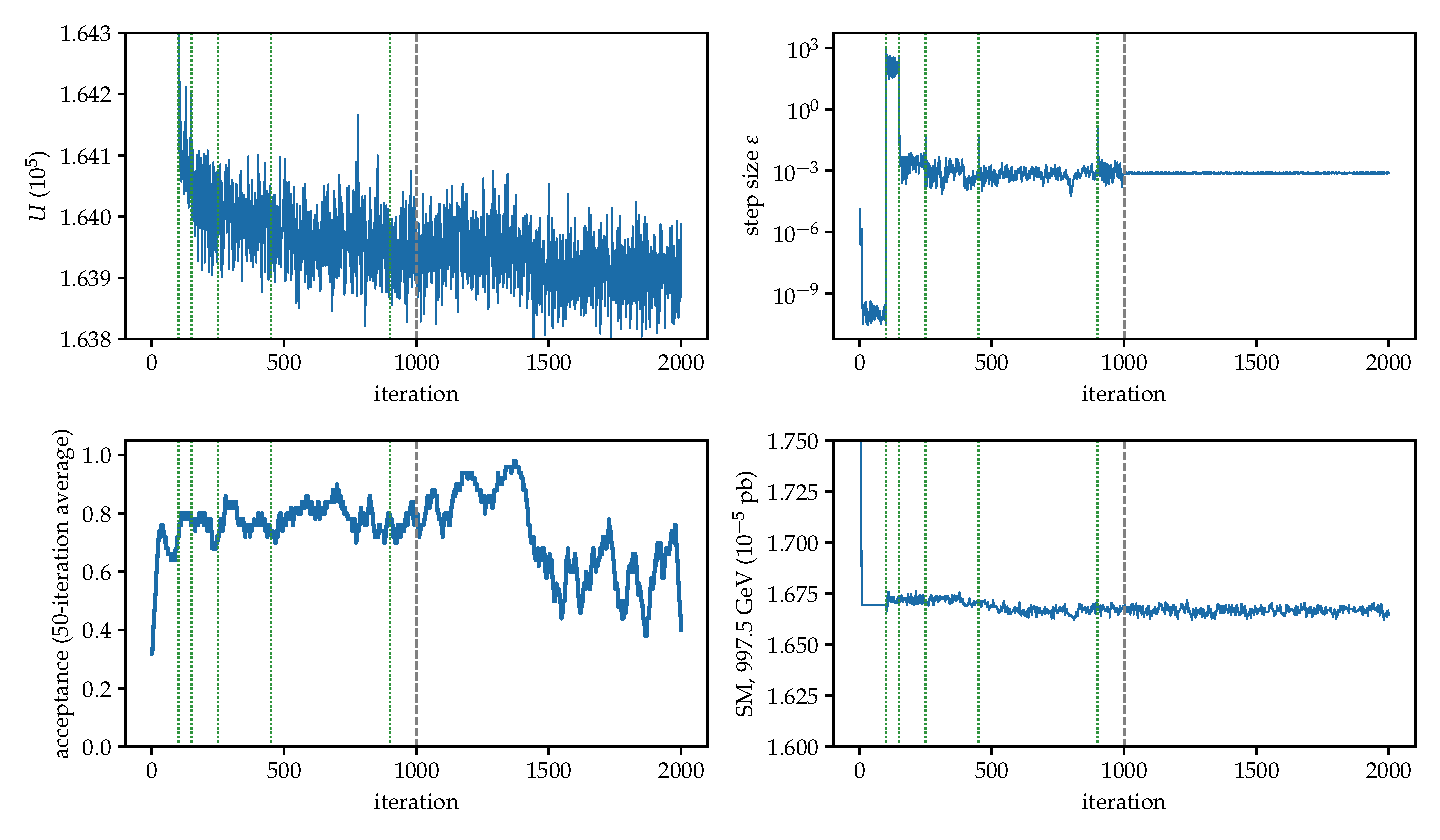
\includegraphics[width=\textwidth]{fig3_traces.pdf}
\caption{The full-data run: $U$, the step size, the acceptance rate (50-iteration running
average) and the SM prediction at 997.5 GeV. Green dotted lines: mass-matrix updates;
grey dashed line: end of the warm-up.}
\label{fig:traces}
\end{figure}

\paragraph{A warm-up glitch.} The chain started far from the $\chi^2$ optimum: $U$ fell
from 213,000 to 164,500 in a few iterations. The trajectories with huge energy errors
during that descent drove the step-size tuning down to about $10^{-10}$, so the chain
barely moved during the first window (iterations 76--100). The variances measured in that
window were close to zero, and after the first update the step size jumped to 100--500
(\cref{fig:traces}). The next two updates (150, 250) repaired it, so no harm was done; but
the warm-up should not depend on luck. \Cref{sec:fixes} describes the fix.

\paragraph{Not quite stationary.} Around iteration 1,400, $U$ fell by about 35 (0.8 of
its standard deviation) to a new level, and at the same, fixed step size the acceptance
rate dropped from 0.85--0.94 to about 0.6; there were two divergences after the warm-up.
The chain moved into a region of different curvature. $U$ has ESS 18 and split-$\hat R$
1.13. The monitored predictions mix well (ESS 139 and 134, split-$\hat R$ 1.01, 1.00), and
all 16 $\tau_g$ now mix well (ESS 640--1,076): with all the data the rescaling drift seen
at 10\% has gone. \code{suggest\_thinning} gives $K = 55$, driven by $U$ alone; for the
predictions $K \approx 7$ suffices.

% ===========================================================================
\section{The bootstrap ensemble}
\label{sec:ensemble}

\begin{itemize}
  \item 20 members, each on 274,152 rows drawn with replacement (63.2\% distinct), 7--9.5
    minutes each on the 5090.
  \item \textbf{Validation versus out-of-bag loss.} Every member's out-of-bag loss (about
    0.0029) is below its validation loss (about 0.0032). This is not leakage: for member 1
    the mean absolute error is 0.00295 on its training rows, 0.00288 on its out-of-bag
    rows and 0.00296 on the quick-test rows, equal within noise. The validation rows simply
    have 15\% larger cross sections on average (0.126 against 0.109 pb), and the L1 error
    grows with the cross section. Equal in-bag and out-of-bag errors also mean that the
    members do not overfit.
  \item \textbf{Members differ most near threshold}: their individual $\chi^2$ per bin at
    255--555 GeV ranges from 3.7 to 8.6 (median 5.5), against a median $\chi^2/N$ of
    1.165 overall. The ensemble mean (4.1) is better than any typical member.
\end{itemize}

% ===========================================================================
\section{Comparison on the holdout spectra}
\label{sec:holdout}

\begin{center}
\small
\begin{tabular}{lcccccc}
\toprule
& med.\ $\chi^2/N$ & $\chi^2/N > 5$ & $\chi^2$/bin, & $\chi^2$/bin, & width / & neg.\\
& & & 255--555 & $> 555$ & noise & pred.\\
\midrule
L1Loss (single) & 1.171 & 4.9\% & 8.4 & 1.20 & --- & 0.18\%\\
ensemble members (median) & 1.165 & & 5.5 & & --- & \\
ensemble mean & 1.118 & 2.2\% & 4.1 & 1.14 & 0.157 & 0.06\%\\
BNN, 10\% (run 3) & 1.090 & 1.1\% & 1.7 & 1.11 & 0.057 & 0.006\%\\
BNN, full data & 1.099 & 1.2\% & 1.9 & 1.12 & 0.005 & 0.03\%\\
\bottomrule
\end{tabular}
\end{center}

\begin{figure}[h]
\centering
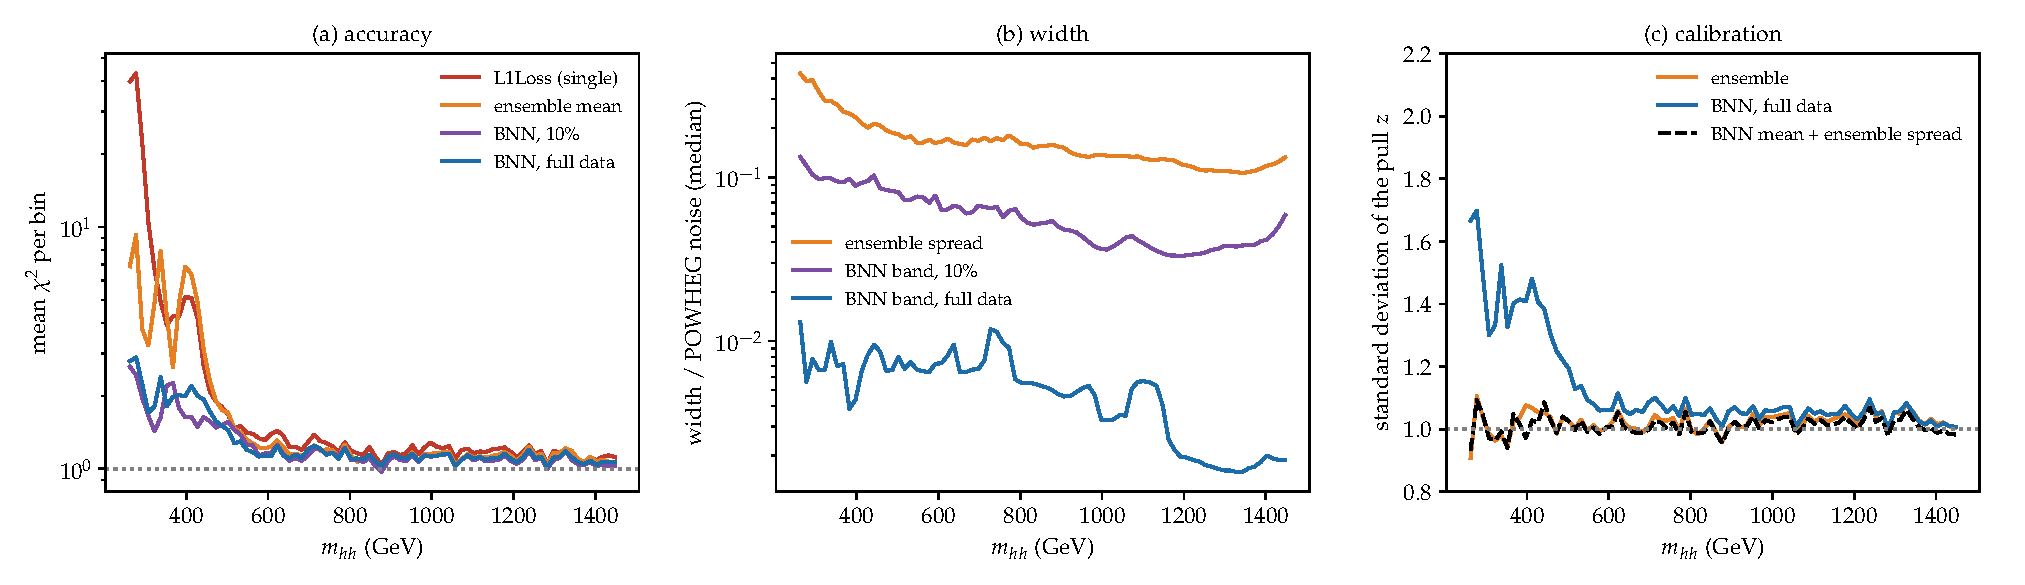
\includegraphics[width=\textwidth]{fig3_holdout.pdf}
\caption{(a) Mean $\chi^2$ per bin against $\mhh$. (b) Width of the uncertainty (ensemble
spread or BNN posterior s.d.) in units of the POWHEG noise. (c) Standard deviation of the
pull $z = (t - \bar f)/\sqrt{\sigma_k^2 + s^2}$ against $\mhh$.}
\label{fig:holdout}
\end{figure}

\begin{center}
\small
\begin{tabular}{lccccc}
\toprule
& pull s.d.: all & 255--555 & $> 555$ & $|z| < 2$ & $|z| > 3$\\
\midrule
ensemble (mean, spread) & 1.025 & 1.020 & 1.026 & 95.0\% & 0.56\%\\
BNN, 10\% & 1.084 & 1.192 & 1.044 & 93.9\% & \\
BNN, full data & 1.143 & 1.370 & 1.055 & 93.5\% & 1.07\%\\
BNN full mean + ensemble spread & 1.014 & 1.014 & 1.015 & 95.2\% & 0.42\%\\
\midrule
standard normal & 1 & 1 & 1 & 95.4\% & 0.27\%\\
\bottomrule
\end{tabular}
\end{center}

\begin{figure}[h]
\centering
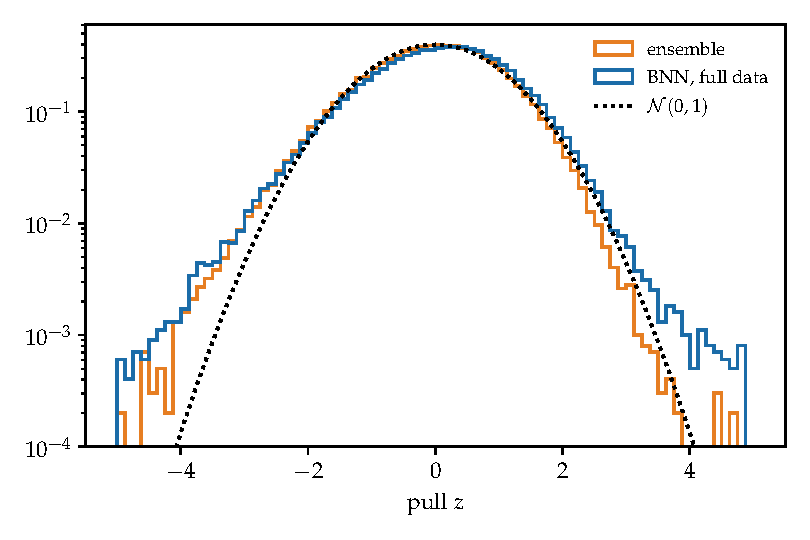
\includegraphics[width=0.6\textwidth]{fig3_pulls.pdf}
\caption{Distribution of the pull over all holdout bins, for the ensemble and the
full-data BNN, against a standard normal.}
\label{fig:pulls}
\end{figure}

\noindent Three observations:
\begin{enumerate}
  \item \textbf{The ensemble's spread is the right size,} in both regions; the core of its
    pull distribution is standard normal (robust s.d.\ from the median absolute deviation:
    1.007). The tails are heavier than Gaussian: 0.56\% of bins have $|z| > 3$ against
    0.27\%, and 0.06\% have $|z| > 4$ against 0.006\% (\cref{fig:pulls}); a few bins are
    badly mismodelled by all members, or have a poorly estimated noise.
  \item \textbf{The full-data BNN band is far too narrow.} It shrank 12-fold from the 10\%
    run, not by $\sqrt{10} \approx 3.2$, and the full-data and 10\% means differ by a
    median of 1.5 of the 10\% run's posterior standard deviations. Each run's band
    describes only the valley it is in. With all the data, the parametric uncertainty of
    one network is negligible; what remains is the variability between equally good
    networks and the model's own error, which the ensemble captures and one HMC chain does
    not.
  \item \textbf{The best mean and the best spread come from different procedures.}
    Combined, they are calibrated everywhere (pull s.d.\ 1.01). The next section proposes
    how to obtain both from one procedure.
\end{enumerate}

% ===========================================================================
\section{Fixes to \texttt{hmc.py}}
\label{sec:fixes}

\begin{itemize}
  \item \textbf{A fresh step size at the end of the initial buffer.} At iteration 75 the
    warm-up now searches for a new step size for the chain as it is, and restarts the
    tuning, so that the first mass-matrix window is not sampled with a step size crippled
    by the early descent.
  \item \textbf{Useless windows are skipped.} If fewer than 3 trajectories were accepted in
    a window, or the measured variances are zero or not finite, the old mass matrix is kept
    (and a message says so).
  \item \textbf{Samples are saved on the CPU,} so that a plain \code{torch.load} reads them
    on a machine without a GPU; \code{BNN.export} converts older, GPU-saved files.
  \item \textbf{Checks.} The toy notebook passes (its correlation check now uses the Monte
    Carlo error of a correlation coefficient, $(1-\rho^2)/\sqrt{n_\text{eff}}$, instead of
    a fixed 0.05; a run with 20,000 samples confirmed that the differences shrink as
    expected); interrupt-and-resume, including at iteration 75 and at a window boundary,
    still gives identical files; a short Poisson run of the BNN notebook works end to end.
    The exact full-data glitch could not be reproduced on a CPU, so the first fix is
    defensive: its effect will be seen in the next full-data run.
\end{itemize}

% ===========================================================================
\section{Towards a publishable result}
\label{sec:paper}

\begin{keyidea}[Proposal]
Make an ensemble the headline result, trained with a \emph{robust, noise-weighted}
loss, and present the BNN as a cross-check. I agree with the idea of using the Huber
loss, with one essential qualification: it should be applied to the residuals in units of
the POWHEG noise, $r_k = (f_k - t_k)/\sigma_k$, not to the residuals in pb.
\end{keyidea}

\paragraph{Why an ensemble as the headline.} It is simple, cheap (20 members in about three
hours on the 5090), easy to reproduce, familiar to readers, and has a clear frequentist
meaning once the reference ensemble is stated (\file{ensemble_plan.pdf}, \S3). Above all,
its calibration has been demonstrated on spectra never used in training. The BNN, by
contrast, needs long chains whose convergence is hard to certify, and with all the data its
band does not describe the error that matters.

\paragraph{Why Huber, and why on the pulls.} The Huber loss with threshold $\delta$,
\[
  \ell_\delta(r) = \begin{cases} \tfrac12 r^2, & |r| \le \delta,\\
  \delta\,\bigl(|r| - \tfrac12\delta\bigr), & |r| > \delta, \end{cases}
\]
is quadratic for small residuals and linear for large ones. Applied to $r_k$ in units of
the noise:
\begin{itemize}
  \item For the bulk of the bins, $|r_k| \lesssim 2$, it \emph{is} $\chi^2$: the weighting
    by precision that brought the threshold $\chi^2$ from 8.4 to 1.9 in the BNN. Applied to
    residuals in pb, as an interpolation between MSE and L1, it would keep their weakness:
    a $10^{-4}$~pb error counts the same in every bin, so the large cross sections dominate
    and the threshold region is neglected.
  \item For bins with large pulls it grows only linearly, so a few mismodelled or
    anomalous bins (the ten incomplete POWHEG runs; the heavy tails of \cref{fig:pulls})
    cannot dominate the fit. Early in training, when many pulls are large, each bin's
    gradient is capped at $\delta/\sigma_k$ instead of growing with its residual, which
    should ease (though not remove: $1/\sigma_k$ still spans several decades) the
    conditioning problem that made the plain CHI2 loss fail.
  \item It ties the story together: the ensemble's loss and the BNN's Poisson likelihood are
    the same $\chi^2$ for well-modelled bins, so the BNN becomes a genuine cross-check of the
    same fit, not of a different one.
\end{itemize}

\paragraph{Training.} The BNN runs showed that a $\chi^2$-type objective works when
started from the L1 solution with full-data gradients, and the earlier CHI2 runs showed
that it fails from scratch with mini-batches of 2,048. The safe recipe is therefore two
stages for every member: the L1 training of \file{heft_train.ipynb}, then a fine-tune with
the Huber-pull loss at large batch size and small learning rate. One design point needs
your decision: the loss needs each row's noise $\sigma_k$, which you do not want as a
second target column. It can be computed from the target $t_k$ and the spectrum's total
cross section, $\sigma_k^2 = (t_k + \sigma_\text{tot}/N_\text{eff})\,\sigma_\text{tot}/N_\text{eff}$,
so what is needed is $\sigma_\text{tot}$ per row, carried alongside the data rather than as
a target.

\paragraph{The steps, in order.}
\begin{enumerate}
  \item \textbf{One model first:} L1 then Huber-pull fine-tune, $\delta \in \{1, 2, 3\}$;
    success if the threshold $\chi^2$ per bin approaches the BNN's 1.9 without losing
    elsewhere. Cheap.
  \item \textbf{The bootstrap ensemble with that recipe;} success if it is as accurate as the
    BNN and as well calibrated as the L1 ensemble.
  \item \textbf{The \code{'seeds'} ensemble with the same recipe,} for the split of the
    variance into optimisation and data parts, which a paper would want.
  \item \textbf{The BNN cross-check:} the full-data Poisson BNN, with the fixed warm-up and
    perhaps two chains; its mean should agree with the ensemble mean within the ensemble
    spread, and its narrow band illustrates that parametric uncertainty is negligible.
\end{enumerate}
I can write a plan for step 1 (and the changes to \file{heft_train.ipynb} or a new
notebook) in the usual form before any code is written.

\end{document}
